
\chapter{YARI-RİJİT BİRLEŞİMLER}

\label{CH2} 

\section{Birleşimlerin Sınıflandırılması}

Bu bölümde, ortak yalıtım düzleminde bulunan sismik yalıtımlı tekli
ve çoklu yapılara ait hareket denklemleri, çalışmada kullanılacak
hali ile yeniden türetilmiş ve ardından hareket denklemlerinin çalışma
kapsamında kullanılan doğrusal olmayan çözüm yöntemine ait detaylar
verilmiştir. Bununla birlikte sismik yalıtımlı yapıların analizinde
kullanılan sönüm modellerine ait detaylar paylaşılmıştır. Ayrıca sismik
yalıtımlı yapıların eşdeğer doğrusal analizine ilişkin tasarım metodolojileri
ilgili yöntem ve yönetmelikler dahilinde açıklanmıştır.

\section{Birleşim Davranışının Modellenmesi}

\label{eom-singlestructure} Nagarajaiah ve diğerleri tarafından sunulan
sismik yalıtımlı tek yapılara ait hareket denklemlerinde, her bir
kat 3 serbestlik derecesi ile ifade edilmektedir \cite{doi:10.1061/(ASCE)0733-9445(1991)117:7(2035)}.
Bu çalışma kapsamında, tek doğrultuda yatay ötelenme serbestlik dereceleri
dikkate alınacaktır. Bu sebeple hareket denklemleri, çalışma kapsamında
kullanılacak sınırlar çerçevesinde detaylı olarak açıklanmıştır. Denklemler,
kütleleri kat hizalarında toplanmış olan ve yalnızca yatay kesme yaylarının
yapı rijitliğini temsil ettiği örnek sismik yalıtımlı sistem üzerinden
türetilmiştir. 
\begin{figure}[h!]
\centering{}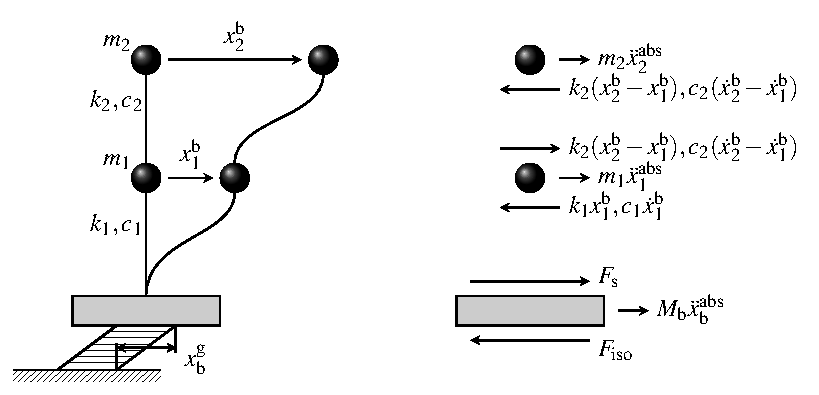
\includegraphics{TikZ/SingleStructureAndFBD} \caption{\label{fig:singlestructurefbd}Sismik yalıtımlı tek yapının şekil
değiştirmiş hali ve serbest cisim diyagramı.}
\end{figure}

Şekil \ref{fig:singlestructurefbd}'de yapının temsili şekil değiştirmiş
hali ile dinamik yükleme altında katlara ve yalıtım düzlemine etkiyen
kuvvetler sunulmuştur. Burada, $x^{\text{b}}$ katların yalıtım düzlemine
göre bağıl yer değiştirmelerini, $x_{\text{b}}^{\text{g}}$ yalıtım
düzleminin zemine göre bağıl yer değiştirmesini, $m$ kat kütlelerini,
$m_{\text{b}}$ yalıtım düzlemi kütlesini, $k$ kat rijitliklerini,
$c$ ilgili kata ait sönüm değerini, $F_{\text{s}}$ yapının taban
kesme kuvvetini, $F_{\text{iso}}$ izolatör seviyesinde oluşan kesme
kuvvetini ve noktalar ise zamana bağlı türevi belirtmektedir. Terimlerde
alt indis şeklinde bulunan numaralar, ilgili büyüklüğün hangi kata
ait olduğunu göstermektedir. Buna göre, yapının ilk katına ait hareket
denklemi \ref{eq-eom-1}'deki gibi ifade edilebilir. 
\begin{equation}
-k_{2}\left[x_{2}^{\text{b}}-x_{1}^{\text{b}}\right]+k_{1}x_{1}^{\text{b}}-c_{2}\left[\dot{x}_{2}^{\text{b}}-\dot{x}_{1}^{\text{b}}\right]+c_{1}\dot{x}_{1}^{\text{b}}=-m_{1}\ddot{x}_{1}^{\text{abs}}\label{eq-eom-1}
\end{equation}
Dinamik denge, D'Alembert prensibine göre yazılmıştır. Bu prensibe
göre, sisteme etkiyen kuvvetlerin yanı sıra, fiktif atalet kuvvetlerinin
ivme yönüne ters olarak eklenmesi halinde sistem her zaman anı için
denge durumunda bulunmaktadır. Dolayısıyla eşitliğin sağ tarafında
yer alan $\ddot{x}_{1}^{\text{abs}}$ terimi, aşağıdaki denklemde
belirtildiği gibi yalıtım düzleminde oluşan ve $\ddot{x}_{\text{b}}^{\text{abs}}$
ile ifade edilen ivmeler ile, dinamik dengenin sağlanabilmesi için
denkleme eklenen fiktif $\ddot{x}_{1}^{\text{b}}$ ivmesinin toplamını
ifade etmektedir. 
\begin{equation}
\ddot{x}_{1}^{\text{abs}}=\ddot{x}_{1}^{\text{b}}+\ddot{x}_{\text{b}}^{\text{abs}}\label{eq-acc-1}
\end{equation}
Benzer şekilde yapının ikinci katına ait hareket denklemi ve $\ddot{x}_{2}^{\text{abs}}$
teriminin açılımı aşağıda sunulmuştur. 
\begin{equation}
k_{2}\left[x_{2}^{\text{b}}-x_{1}^{\text{b}}\right]+c_{2}\left[\dot{x}_{2}^{\text{b}}-\dot{x}_{1}^{\text{b}}\right]=-m_{2}\ddot{x}_{2}^{\text{abs}}\label{eq-eom-2}
\end{equation}
\begin{equation}
\ddot{x}_{2}^{\text{abs}}=\ddot{x}_{2}^{\text{b}}+\ddot{x}_{\text{b}}^{\text{abs}}\label{eq-acc-2}
\end{equation}
Yukarıda verilen denklemler düzenlenerek matris formunda yazılırsa
aşağıda sunulan denklem elde edilir. 
\begin{equation}
\begin{split}\begin{bmatrix}m_{1} & 0\\
0 & m_{2}
\end{bmatrix}\begin{Bmatrix}\ddot{x}_{1}^{\text{b}}\\
\ddot{x}_{2}^{\text{b}}
\end{Bmatrix}+ & \begin{bmatrix}c_{1}+c_{2} & -c_{2}\\
-c_{2} & c_{2}
\end{bmatrix}\begin{Bmatrix}\dot{x}_{1}^{\text{b}}\\
\dot{x}_{2}^{\text{b}}
\end{Bmatrix}+\begin{bmatrix}k_{1}+k_{2} & -k_{2}\\
-k_{2} & k_{2}
\end{bmatrix}\begin{Bmatrix}{x}_{1}^{\text{b}}\\
{x}_{2}^{\text{b}}
\end{Bmatrix}=\\
 & -\begin{bmatrix}m_{1} & 0\\
0 & m_{2}
\end{bmatrix}\begin{Bmatrix}1\\
1
\end{Bmatrix}\ddot{x}_{\text{b}}^{\text{abs}}
\end{split}
\label{eq-eom-singlestructure}
\end{equation}
Aşağıdaki denklemde açıklandığı üzere $\ddot{x}_{\text{b}}^{\text{abs}}$
terimi, $\ddot{x}_{\text{b}}^{\text{g}}$ ile ifade edilen yalıtım
düzleminin zemine göre bağıl ivmesi ile $\ddot{x}_{\text{g}}^{\text{abs}}$
ifadesine karşılık gelen yer ivmesinin toplamını belirtmektedir. 
\begin{equation}
\ddot{x}_{\text{b}}^{\text{abs}}=\ddot{x}_{\text{b}}^{\text{g}}+\ddot{x}_{\text{g}}^{\text{abs}}\label{eq-abs-base-acc}
\end{equation}
Yalıtım düzlemine göre bağıl olarak ifade edilmiş olan yapının hareket
denklemi kapalı formda aşağıdaki gibi yazılabilir. 
\begin{equation}
\mathbf{M}_{\text{s}}\mathbf{\ddot{x}}_{\text{s}}^{\text{b}}+\mathbf{C}_{\text{s}}\mathbf{\dot{x}}_{\text{s}}^{\text{b}}+\mathbf{K}_{\text{s}}^{\text{b}}\mathbf{x}_{\text{s}}^{\text{b}}=-\mathbf{M}_{\text{s}}\mathbf{R}\ddot{x}_{\text{b}}^{\text{g}}-\mathbf{M}_{\text{s}}\mathbf{R}\ddot{x}_{\text{g}}^{\text{abs}}\label{eq-eom-singlestructure-closed}
\end{equation}
Burada, $\mathbf{M}_{\text{s}}$ kütle, $\mathbf{C}_{\text{s}}$ sönüm,
$\mathbf{K}_{\text{s}}$ rijitlik matrisini, $\mathbf{x}_{\text{s}}$
katların yalıtım düzlemine göre bağıl yer değiştirme vektörünü, $\mathbf{\ddot{x}}_{\text{b}}^{\text{g}}$
yalıtım düzleminin zemine göre bağıl ivmesini, $\mathbf{\ddot{x}}_{\text{g}}^{\text{abs}}$
yer ivmesini, $\mathbf{R}$ deprem etki vektörünü ve noktalar ise
zamana bağlı türevleri ifade etmektedir. Elde edilen üst yapı bağıl
hareket denkleminde deprem kuvvetlerini oluşturacak ivmeler, yalnızca
yalıtım düzleminin mutlak ivmesine eşittir. Dolayısıyla üst yapıya
etkiyen deprem kuvvetlerinde yer ivmelerinin doğrudan etkisi bulunmamaktadır.

Burada, $\mathbf{M}$, $\mathbf{C}$ ve $\mathbf{K}$ tüm yapıya ait
sırasıyla kütle, sönüm ve rijitlik matrislerini, $\mathbf{x}$ yapı
yer değiştirme vektörünü ve $\mathbf{S}_{\text{1}}$ ise etki vektörünü
ifade etmektedir. Denklemde belirtilen terimlerin açık hali aşağıda
verilmiştir. \vspace{0.2cm}

\begin{center}
$\mathbf{M}=\begin{bmatrix}\mathbf{M}_{\text{s}} & \mathbf{M}_{\text{s}}\mathbf{R}\\
\mathbf{R}^{\text{T}}\mathbf{M}_{\text{s}} & \mathbf{R}^{\text{T}}\mathbf{M}_{\text{s}}\mathbf{R}+M_{\text{b}}
\end{bmatrix}$ \hspace{0.2cm} $\mathbf{M}_{\text{s}}=\begin{bmatrix}m_{1} & 0\\
0 & m_{2}
\end{bmatrix}$ \vspace{0.25cm}
\par\end{center}

\begin{center}
$\mathbf{C}=\begin{bmatrix}\mathbf{C}_{\text{s}} & \mathbf{0}\\
\mathbf{0} & C_{\text{b}}
\end{bmatrix}$ \hspace{0.2cm} $\mathbf{C}_{\text{s}}=\begin{bmatrix}c_{1}+c_{2} & -c_{2}\\
-c_{2} & c_{2}
\end{bmatrix}$ \vspace{0.25cm}
\par\end{center}

\begin{center}
$\mathbf{K}=\begin{bmatrix}\mathbf{K}_{\text{s}} & \mathbf{0}\\
\mathbf{0} & K_{\text{b}}
\end{bmatrix}$ \hspace{0.2cm} $\mathbf{K}_{\text{s}}=\begin{bmatrix}k_{1}+k_{2} & -k_{2}\\
-k_{2} & k_{2}
\end{bmatrix}$ \vspace{0.25cm}
\par\end{center}

\begin{center}
$\mathbf{\ddot{x}}=\begin{Bmatrix}\mathbf{\ddot{x}}_{\text{s}}^{\text{b}}\\
\ddot{x}_{\text{b}}^{\text{g}}
\end{Bmatrix}$ \hspace{0.2cm} $\mathbf{\ddot{x}}_{\text{s}}^{\text{b}}=\begin{Bmatrix}\ddot{x}_{1}^{\text{b}}\\
\ddot{x}_{2}^{\text{b}}
\end{Bmatrix}$ \hspace{0.5cm} $\mathbf{\dot{x}}=\begin{Bmatrix}\mathbf{\dot{x}}_{\text{s}}^{\text{b}}\\
\dot{x}_{\text{b}}^{\text{g}}
\end{Bmatrix}$ \hspace{0.2cm} $\mathbf{\dot{x}}_{\text{s}}^{\text{b}}=\begin{Bmatrix}\dot{x}_{1}^{\text{b}}\\
\dot{x}_{2}^{\text{b}}
\end{Bmatrix}$ \hspace{0.5cm} $\mathbf{x}=\begin{Bmatrix}\mathbf{x}_{\text{s}}^{\text{b}}\\
{x}_{\text{b}}^{\text{g}}
\end{Bmatrix}$ \hspace{0.2cm} $\mathbf{x}_{\text{s}}^{\text{b}}=\begin{Bmatrix}{x}_{1}^{\text{b}}\\
{x}_{2}^{\text{b}}
\end{Bmatrix}$ \vspace{0.25cm}
\par\end{center}

\begin{center}
$\mathbf{S}_{\text{1}}=\begin{Bmatrix}\mathbf{0}\\
1
\end{Bmatrix}$ \hspace{0.2cm} $\mathbf{R}=\begin{Bmatrix}1\\
1
\end{Bmatrix}$ 
\par\end{center}

\newpage{}

\section{Birleşim Dönme Kapasitesi}

Sismik yalıtımlı çoklu yapılara ait hareket denklemleri Tsopelas ve
diğerleri tarafından açıklanmıştır \cite{TSOPELAS199447}. Yapılan
çalışmada, düzlem içi rijitlikleri sonsuz yapı katlarını temsil eden
toplu kütlelerin iki yatay ötelenme ve bir dönme olmak üzere toplam
üç adet serbestlik derecesi bulunmaktadır. Kütle merkezlerinde konumlanan
bu serbestlik dereceleri, yalıtım düzlemi kütle merkezinden geçen
düşey referans aksa göre eksantrik olarak tanımlanabilmektedir. Tez
çalışması kapsamında ortak yalıtım düzleminde bulunan çoklu yapıların
parametrik değişkenler altında yapı davranışları, yalnızca tek doğrultuda
yatay ötelenme serbestlik dereceleri dikkate alınarak incelenmiştir.
Bu sebeple hareket denklemleri, Şekil \ref{fig:multistructure}'de
sunulan örnek yapı üzerinden türetilecektir.

\section{Önceki Çalışmalar}

\begin{figure}[h]
\centering{}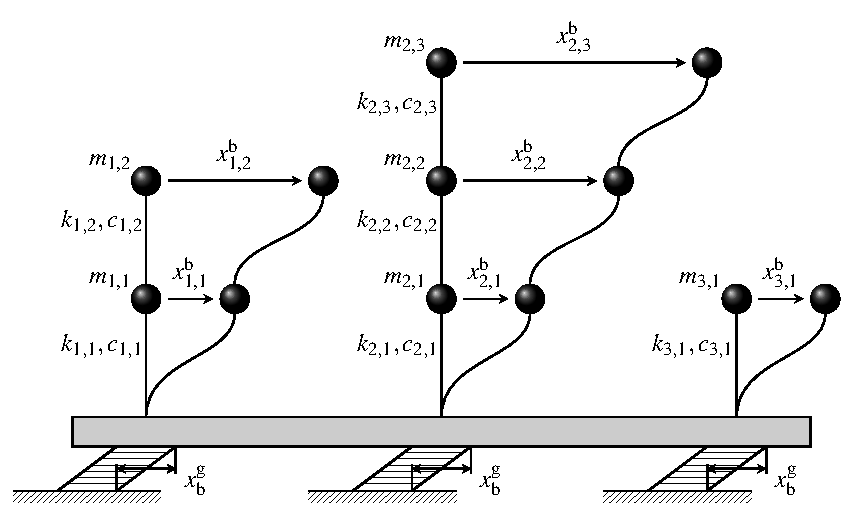
\includegraphics[width=1\linewidth]{TikZ/MultiStructure}
\caption{\label{fig:multistructure}Sismik yalıtımlı çoklu yapıların şekil
değiştirmiş hali.}
\end{figure}

Burada, $m$ kat kütlelerini, $c$ kat sönümünü, $k$ rijitlik değerini
ve $x$ ise yer değiştirmeleri belirtmektedir. Üst indiste büyüklüğün
göreli olarak yazıldığı konum belirtilmiştir. Yapı kat yer değiştirmelerinde
alt indislerde verilen ilk rakam yapı numarasını, ikinci rakam ise
büyüklüğün hangi kata ait olduğunu işaret etmektedir. Yalıtım düzlemi
yer değiştirmesi veya izolatör deplasmanları ise $x_{\text{b}}^{\text{g}}$
ile verilmiştir.
